\documentclass[fontset=windows,a4paper,oneside,10pt]{article}

\usepackage{./packages/resume}

% \setmainfont[
%   Path = support/config/fonts/Main/,
%   Extension = .otf,
%   UprightFont = *-regular,
%   BoldFont = *-bold,
%   ItalicFont = *-italic,
%   BoldItalicFont = *-bolditalic,
%   SmallCapsFont = Fontin-SmallCaps
% ]{texgyretermes}

% % 设置默认的字体路径和字体
% \defaultfontfeatures{Path = support/config/fonts/zh_CN-Adobe/, Mapping=tex-text}

% % 设置 CJK 字体
% \setCJKmainfont[
%   BoldFont=AdobeHeitiStd-Regular.otf,
%   ItalicFont=AdobeKaitiStd-Regular.otf,
%   SmallCapsFont=AdobeHeitiStd-Regular.otf
% ]{AdobeSongStd-Light.otf}

% \setCJKsansfont{AdobeHeitiStd-Regular.otf}
% \setCJKmonofont{AdobeFangsongStd-Regular.otf}

% \setCJKfamilyfont{zhsong}{AdobeSongStd-Light.otf}
% \setCJKfamilyfont{zhhei}{AdobeHeitiStd-Regular.otf}
% \setCJKfamilyfont{zhfs}{AdobeFangsongStd-Regular.otf}
% \setCJKfamilyfont{zhkai}{AdobeKaitiStd-Regular.otf}

% % 定义常用字体命令
% \newcommand{\songti}{\CJKfamily{zhsong}} % 宋体
% \newcommand{\heiti}{\CJKfamily{zhhei}}   % 黑体
% \newcommand{\kaishu}{\CJKfamily{zhkai}}  % 楷书
% \newcommand{\fangsong}{\CJKfamily{zhfs}} % 仿宋

\setmainfont{TeX Gyre Termes}

\defaultfontfeatures{Mapping=tex-text}

\setCJKmainfont[
  BoldFont=Adobe Heiti Std R,
  ItalicFont=Adobe Kaiti Std R,
  SmallCapsFont=Adobe Heiti Std R
]{Adobe Song Std L}

\setCJKsansfont{Adobe Heiti Std R}
\setCJKmonofont{Adobe Fangsong Std R}

\setCJKfamilyfont{zhsong}{Adobe Song Std L}
\setCJKfamilyfont{zhhei}{Adobe Heiti Std R}
\setCJKfamilyfont{zhfs}{Adobe Fangsong Std R}
\setCJKfamilyfont{zhkai}{Adobe Kaiti Std R}

\newcommand{\songti}{\CJKfamily{zhsong}} % 宋体
\newcommand{\heiti}{\CJKfamily{zhhei}}   % 黑体
\newcommand{\kaishu}{\CJKfamily{zhkai}}  % 楷书
\newcommand{\fangsong}{\CJKfamily{zhfs}} % 仿宋

\begin{document} 

\pagenumbering{gobble}

\begin{center}
    \begin{minipage}[c]{0.15\textwidth}
        \begin{figure}[H]
            \raggedright
            % \vspace*{-5ex}
            
\includegraphics[width=\linewidth]{./figures/avatar.jpg}
        \end{figure}
    \end{minipage}
    \hfill
    \begin{minipage}[c]{0.6\textwidth}
        \begin{figure}[H]
            \Large
            \begin{tabular}{cl}
                {\faUser}&\name{你的名字} \\
                {\faEnvelope}&\email{你的邮箱} \\
                {\faPhone}&\phone{你的电话号码}
            \end{tabular}
        \end{figure}
    \end{minipage}
    \hfill
    \begin{minipage}[c]{0.2\textwidth}
        \begin{figure}[H]
            \raggedleft
            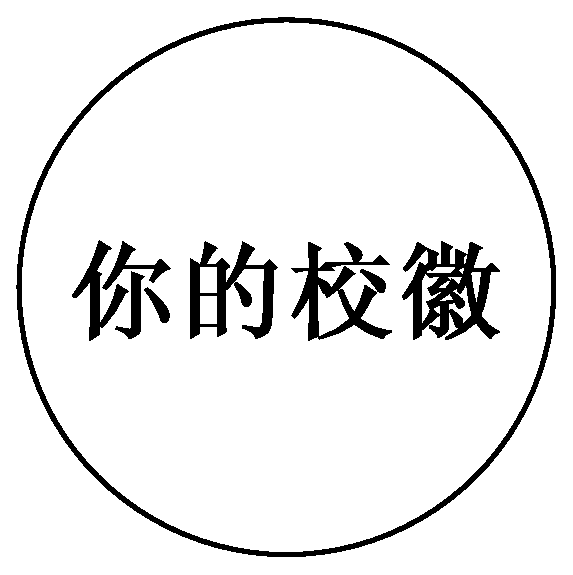
\includegraphics[width=0.8\textwidth]{./figures/your_logo.eps}
        \end{figure}
    \end{minipage}
\end{center}

% \basicInfo{}

\section{\faGraduationCap\  教育背景}
\datedsubsection{\textbf{你的学校}}{起止日期}
\textit{2022级本科生在读}\quad 你的学院(系)\quad 你的专业
\begin{itemize}[parsep=0.5ex]
	\item 成绩排名\qquad  GPA\ (你的GPA) \quad 平均学分绩\ (你的平均学分绩) \quad 专业排名\ (你的专业排名)
	\item 主干课程\qquad  课程\ 分数\quad 课程\ 分数 \quad 课程\ 分数 \quad 课程\ 分数
	\item 英语水平\qquad  CET4\ 分数 \quad CET6\ 分数
\end{itemize}

\section{\faEye\ 科研经历} %\faLightbulbO

\datedsubsection{\textbf{科研经历1}\quad {\normalsize 指导教师or所在单位or其他}}{起止日期}
\begin{onehalfspacing}
\begin{itemize}[parsep=0.5ex]
  \item 你的工作
  \item 你的工作
  \item 你的工作
\end{itemize}
\end{onehalfspacing}

\datedsubsection{\textbf{科研经历2}\quad {\normalsize 指导教师or所在单位or其他}}{起止日期}
\begin{onehalfspacing}
\begin{itemize}[parsep=0.5ex]
  \item 你的工作
  \item 你的工作
  \item 你的工作
  \item 你的工作
\end{itemize}
\end{onehalfspacing}

\section{\faTrophy\ 获奖情况}
\begin{itemize}[parsep=0.5ex]
  \item \datedline{你的奖(学金)名称}{获奖时间}
  \item \datedline{你的奖(学金)名称}{获奖时间}
  \item \datedline{你的奖(学金)名称}{获奖时间}
  \item \datedline{你的奖(学金)名称}{获奖时间}
\end{itemize}

\section{\faCogs\ 其他技能}
% increase linespacing [parsep=0.5ex]
\begin{itemize}[parsep=0.5ex]
  \item 你的技能
  \item 你的技能
\end{itemize}

\end{document}
